\chapter{G\lowercase{a}A\lowercase{s} activation with C\lowercase{s}-T\lowercase{e}}
\section{Abstract}
Photocathodes capable of providing high intensity and highly spin-polarized electron beams with long operational lifetimes are of great interest for the next generation nuclear physics facilities like Electron Ion Colliders. We report on GaAs photocathodes activated by Cs$_2$Te, a material well known for its robustness. GaAs activated by Cs$_2$Te forms Negative Electron Affinity, and the lifetime for extracted charge is improved by a factor of 5 compared to that of GaAs activated by Cs and O$_2$. The spin polarization of photoelectrons was measured using a Mott polarimeter and found to be independent from the activation method, thereby shifting the paradigm on spin-polarized electron sources employing photocathodes with robust coatings.

\section{Introduction}
As of today, the operational lifetime of GaAs-based photocathodes remains a primary limit to the production of highly spin-polarized electron beams with high average currents. Such beams are essential to reach design luminosity for future facilities, such as the Electron Ion Collider \cite{eic}, aimed at studying a wide range of phenomena from strong and electro-weak interactions to physics beyond the Standard Model \cite{lrpns,nsac,mccarter2014_MeasurementElectronBeam}.

Almost all electron sources for highly spin-polarized electron beams in accelerator physics rely on photocathode materials based on GaAs technology. By exposing the GaAs surface to a small quantity of cesium and an oxidant (oxygen or NF$_3$ gases are commonly used) \cite{ciccacci1991_ComparativeStudyPreparation}, a strong dipole moment is formed at the surface that decreases the potential barrier of the electron emission into the vacuum. If the GaAs is also p-doped, due to downward pinning of the bands near the surface, the vacuum level can be lowered below the GaAs conduction band minimum (CBM) achieving the so called Negative Electron Affinity (NEA). When the NEA condition is reached, electrons that have relaxed to the bottom of the conduction band can still escape into the vacuum when they reach the surface. Such condition of GaAs results in a high Quantum Efficiency (QE) even for electrons that are excited with photon energies slightly larger than the band gap \cite{pierce1980_GaAsSpinPolarized}.

The generation of spin-polarized photoelectrons from GaAs takes advantages of the selection rule which conserves the total angular momentum during transitions from the valence band to the conduction band. Due to the degeneracy of the heavy-hole and light-hole band in the P$_{3/2}$ valence band state, a bulk GaAs can provide up to 50\% degree of polarization depending on the doping density.\cite{liu2017_ComprehensiveEvaluationFactors}
Several approaches have been considered to increase the degree of electron spin polarization, the most effective being implementation of a lattice strain in GaAs aimed at breaking the energy degeneracy of the light and the heavy hole bands. Indeed, strained GaAs layers grown on GaAsP produce high polarization up to 90\% by splitting the degenerate energy levels at a cost of decreased QE (0.07\%) using a photon energy of 1.48 eV.\cite{maruyama1992_ElectronspinPolarizationPhotoemission} 
Very recently, GaAs/GaAsP multi-layer super-lattices with a distributed Bragg reflector structure successfully showed an enhanced QE of 6.4\% with a high polarization of 84\%.\cite{liu2016_RecordlevelQuantumEfficiency} 

NEA GaAs photocathodes are notorious for their exceptional vacuum sensitivity. Because activation layers are extremely vulnerable to chemical reactions and weakly bound to the bulk, they require extreme high vacuum (XHV) conditions to survive a long enough time to be of any practical use. Mainly three mechanisms are responsible for the surface degradation of GaAs activated to NEA: ion back-bombardment,\cite{grames2011_ChargeFluenceLifetime} chemical poisoning,\cite{chanlek2014_DegradationQuantumEfficiency} and thermal desorption of the activation layer.\cite{kuriki2011_DarklifetimeDegradationGaAs}
The degradation of photocathode lifetime due to ion back-bombardment is proportional to the overall charge extracted from the cathode. It can be mitigated by extracting electrons from a spot several mm off the electrostatic center of the electron gun.\cite{grames2011_ChargeFluenceLifetime} The advantages of operating under such experimental conditions have been demonstrated in the case of GaAs as well as alkali antimonides.\cite{cultrera2011_PhotocathodeBehaviorHigh,mammei2013_ChargeLifetimeMeasurements}
When NF$_3$ is used as an oxidant, it was reported that activation performed using Cs and Li simultaneously can lead to improved lifetimes.\cite{sun2009_SurfaceActivationLayer,mulhollan2008_EnhancedChemicalImmunity} These studies suggest that chemically stable activation layers can enhance operational lifetime and improve photocathode's ability to better withstand both ion back-bombardment and chemical poisoning.

Cs$_2$Te is a well known solar-blind photocathode material. Its resistance to chemical poisoning and poor vacuum conditions is much larger than that of GaAs. Therefore, it is the most commonly used high-QE photocathode in normal conducting RF guns known for their poorer vacuum.\cite{michelato2008_Cs2TePHOTOCATHODESROBUSTNESS}
Recent studies showed that Cs$_2$Te can also form NEA on GaAs due to a peculiar alignment of the electronic bands of the two materials as shown in Figure \ref{levels} \cite{kuriki2015_GaAsPhotocathodeActivation,sugiyama2011_StudyElectronAffinity,uchida2014_STUDYROBUSTNESSNEAGAAS}.
\begin{figure}
    \centering
    \includegraphics[scale=0.34]{figs/CsTe/levels.pdf}
    \caption{Energy band diagram of GaAs with Cs$_2$Te activation layer. If near IR light ($\sim$ 1.43 eV) is illuminating the sample, the photoelectrons are excited from the GaAs valence band because electrons in Cs$_2$Te require 3.5 eV to reach the vacuum level. NEA is formed on the surface because the vacuum level ($E_{vac}$) is below the GaAs conduction band minimum.}
    \label{levels}
\end{figure}

In this work, we report a NEA condition produced on bulk GaAs using a Cs$_2$Te activation layer, the polarization measurements, and the charge lifetime obtained for these photocathodes. Our results demonstrate a more stable NEA surface as compared to the traditional activation using Cs and O$_2$ without negatively affecting the spin polarization of photoemitted electrons.


Several different specimens were prepared from the same highly p-doped (Zn $5\times10^{18}$ cm$^{-3}$) GaAs (100) wafer.
In order to remove the native oxide layer, a wet etch was performed in a 4\% HCl solution for 5 minutes under the hood in the air. Then, samples were rinsed in deionized water, dried using pure nitrogen, connected to the sample holder, and loaded under vacuum in less than 1 hour. A mild sample heating at about 400 $^\circ$C for 12 hours was deemed sufficient to yield a surface clean enough to perform our experiments. This was inferred from observing that after the heating, the samples could be activated to NEA using only Cs (photoemission observed with $\sim$1.43 eV photons). 
The growth of Cs$_2$Te was performed in a ultra-high vacuum (UHV) chamber equipped with effusion cells hosting BN crucibles loaded with Cs (99.5\% from Strem Chemicals) and Te (99.999\% from Sigma-Aldrich). Each source is equipped with a shutter that allows to trigger on and off the flux towards the substrate surface. After the heat cleaning, the temperature of the samples was lowered to approximately 130 $^\circ$C, and the light of a small diode laser operating at 532 nm was used to illuminate the negatively biased photocathode surface.
\begin{figure}
    \centering
    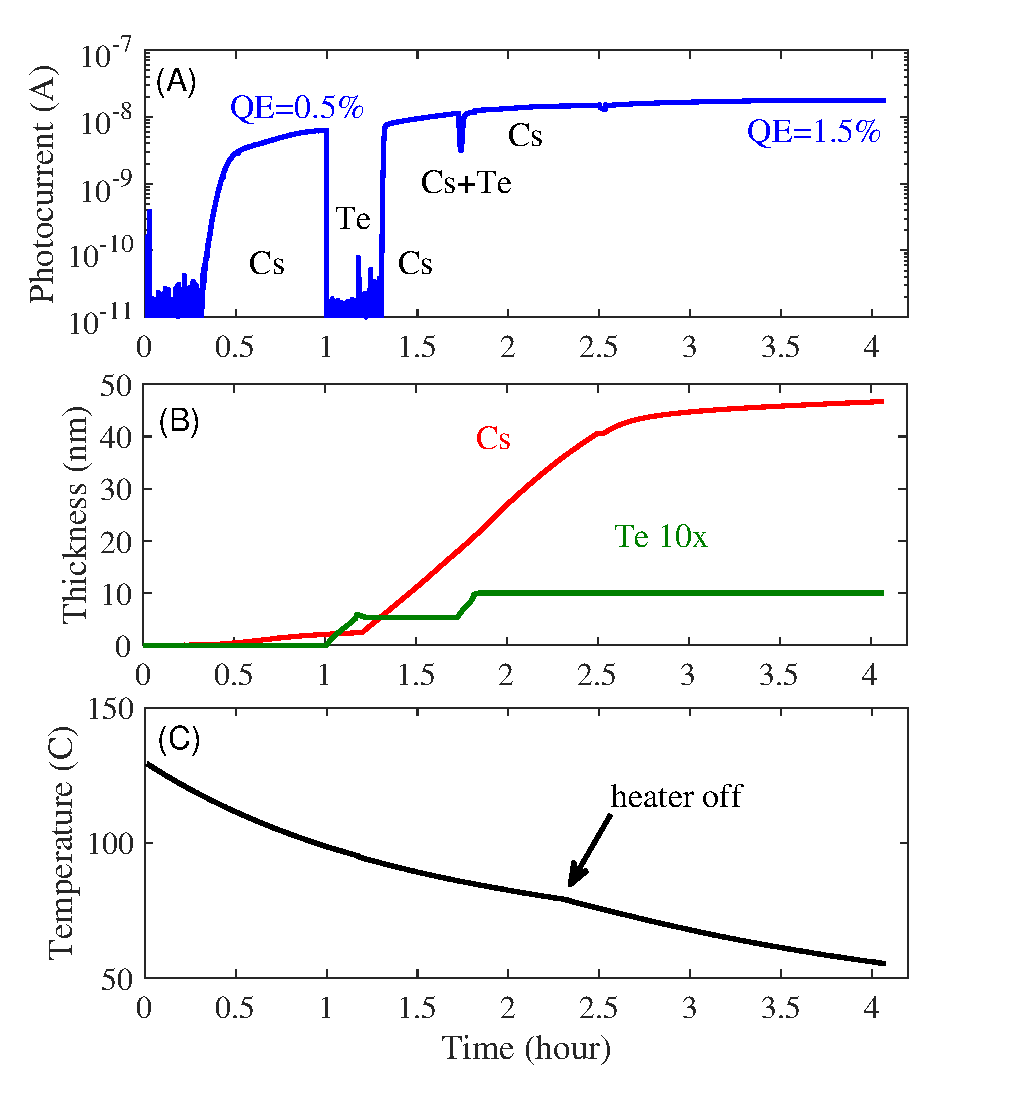
\includegraphics[scale=0.56]{figs/CsTe/growth.eps}
    \caption{(A) Photocurrent measured over time with a 532 nm laser illuminating GaAs during alternating exposure to Cs and Te evaporation; (B) Estimated thicknesses of Cs and Te from the quartz microbalance frequency shift; (C) GaAs substrate temperature during the growth of Cs$_2$Te.}
    \label{growth}
\end{figure}
The Cs$_2$Te growth on GaAs was performed while continuously cooling down the sample from the initial temperature of about 130 $^\circ$C (see Figure \ref{growth} (C)). 
Initially, (see Figure \ref{growth} (A) and (B)) only a small flux of Cs was evaporated until the photocurrent is saturated for an equivalent QE of about 0.5\%, which demonstrates sufficient cleanliness of the GaAs surface. At this point, the shutter for Cs was closed and the one for Te was opened. A sharp decrease of the photocurrent was observed, followed by deposition of 0.5 nm thick Te layer as estimated from the quartz microbalance frequency shift (Figure \ref{growth} (B)). Another Cs deposition followed. The photocurrent increased again until an equivalent QE of about 1\% was reached. A subsequent simultaneous evaporation of Cs and Te (which adds the equivalent of another 0.5 nm of Te) did not improve QE much further (Figure \ref{growth} (A) and (B)). Upon final cooling down, the samples were exposed to a very small flux of Cs reaching a typical final QE of about 1.5\% at 532 nm. %The simultaneous use of sequential deposition and co-depostion was aimed at ensuring that Te was effectively incorporated into the thin surface layer. 

One of the samples was moved under UHV into our surface analysis chamber to analyze the surface by collecting the Auger spectrum (Figure \ref{auger}). The Auger spectra clearly show the distinctive peaks of Te and Cs confirming the presence of the two elements over the GaAs surface.
\begin{figure}
    \centering
    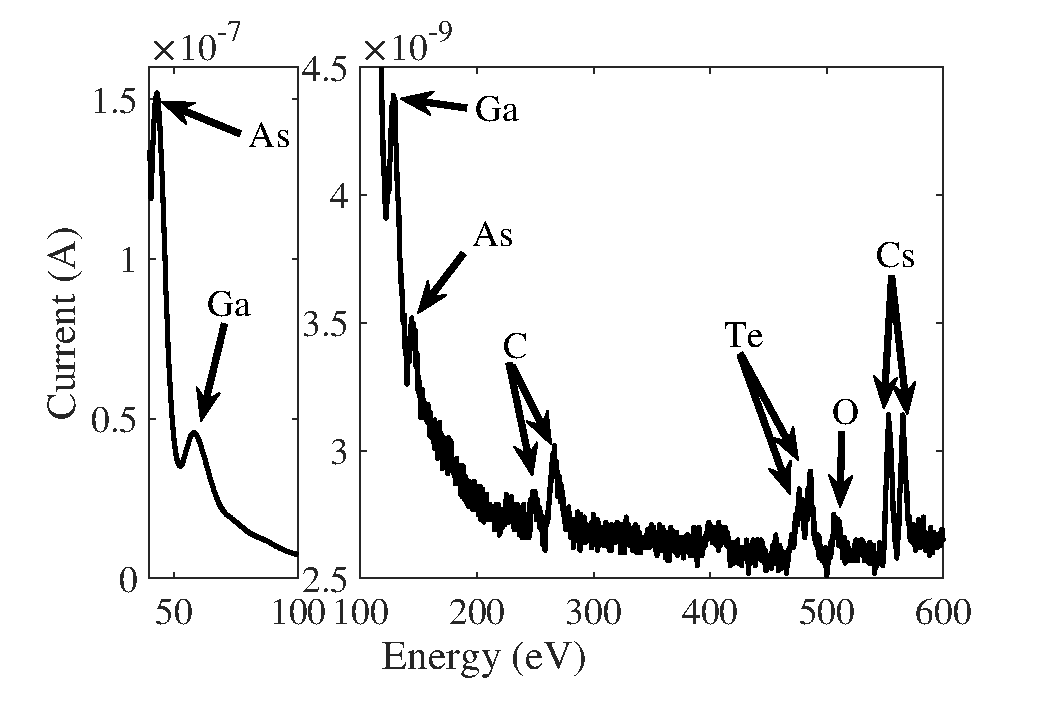
\includegraphics[scale=0.53]{figs/CsTe/auger.eps}
    \caption{Auger electron spectra of GaAs with Cs$_2$Te activation layer.}
    \label{auger}
\end{figure}
Detection of Auger electrons from Ga and As also confirm that the Cs and Te layers are only few nm thick. 

% Spectral response 
The NEA condition was experimentally verified from the spectral response measurements of QE using a broadband lamp and a monochromator. Figure \ref{spectral} shows a typical spectral response from one of our GaAs samples activated with Cs$_2$Te, comparing it with a similar result reported in literature.\cite{kuriki2015_GaAsPhotocathodeActivation} The photoemission at the photon energy of 1.43 eV (the band gap of GaAs), supports the conclusion that the NEA condition is achieved at the surface.

\begin{figure}
    \centering
    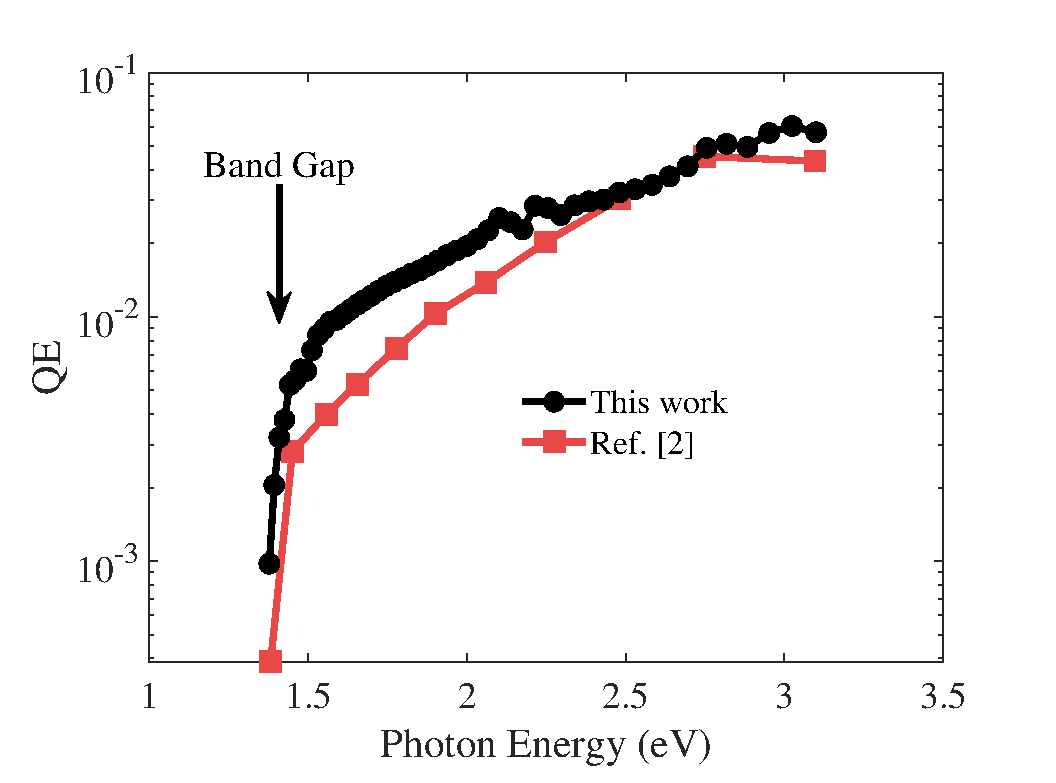
\includegraphics[scale=0.53]{figs/CsTe/spectral.eps}
    \caption{Typical spectral response of our GaAs-Cs$_2$Te as compared to the one from Ref.\cite{kuriki2015_GaAsPhotocathodeActivation}}
    \label{spectral}
\end{figure}

% charge lifetime
Two different metrics are often used for lifetime of a photocathode: operational lifetime, defined as the amount of time a photocathode can satisfy the QE requirement for a particular purpose, and charge lifetime, defined as the amount of charges extracted until QE drops to $1/e$ of the initial value.\cite{grames2011_ChargeFluenceLifetime} The latter has been suggested as a more appropriate figure of merit when comparing the performance of different photocathodes. %fluence lifetime
%ionization cross section, recesiation
In Figure \ref{lifetime}, all lifetime measurements were performed under very similar vacuum conditions (better than $1\times10^{-10}$ Torr) using a 532 nm laser light excitation ($\sim{50} \mu$W) with identical spot size for all illuminations. After each Cs$_2$Te growth, the photocurrent of each sample was constantly measured until the QE went to the $1\times10^{-3}$ level or below. Once such level was reached, the samples were exposed to a Cs flux using alkali-chromate-based dispensers to restore the initial efficiency. QEs were monitored also for the recesiated samples, and all the results are reported in Figure \ref{lifetime}.

The sample coated with an activation layer grown with a 1.2-nm thin film of Te showed the largest charge lifetime value of $9.4\times10^{-3}$  Coulomb. At the same time, the QE at 532 nm was measured to be a factor of 2 larger than the one obtained when a 1.0-nm Te thin film was used. 
%More detailed study of Te thickness on QE of GaAs photocathode was done earlier.\cite{kuriki} 
Compared to the lifetime of $1.9\times10^{-3}$ Coulomb measured for a GaAs activated with Cs and O$_2$, the Cs$_2$Te layer enhanced the lifetime by a factor of 5 in our experimental conditions.
While the exposure to Cs vapors was effective in restoring QEs to even higher levels than the original ones, the charge lifetimes of the recesiated samples are considerably shorter than the original ones. The recesiated samples had charge lifetimes comparable to those of the Cs and O$_2$ activated ones. This suggests that Cs atoms did not penetrate deeply and/or react with the Cs$_2$Te layer but rather deposited on the surface after the recesiation.

Despite the fact that our experiments were performed under UHV conditions, all the charge lifetimes that were measured appear orders of magnitude lower than those reported for GaAs activated to NEA that operated in one of the CEBAF electron guns with a beam energy of 100 keV.\cite{sinclair2007_DevelopmentHighAverage} A simple explanation to this experimental result is related to the vastly different experimental conditions we had in our case. Indeed, unlike the CEBAF gun where the electron beam is accelerated to 100 keV, photoelectrons in our setup are accelerated to mere $\sim$40 eV. At such low kinetic energies, the electron impact ionization cross-section for molecular hydrogen (which is considered to be the dominant chemical species in the residual gas of the vacuum chamber) is 3 orders of magnitude greater than that at 100 keV.\cite{grames2011_ChargeFluenceLifetime,sinclair2007_DevelopmentHighAverage} Also, due to the lack of any deflecting fields, electrons and ions trajectories are co-linear, so that the flux of back-streaming ions is likely to impact at the exact location where the laser spot is illuminating the photocathode. Finally, the positive ions are accelerated at relatively low energies, and hence they will mostly damage a very shallow region near the surface rather than penetrating deeper into the bulk, i.e. affecting the layers responsible for the NEA more effectively.
\begin{figure}
    \centering
    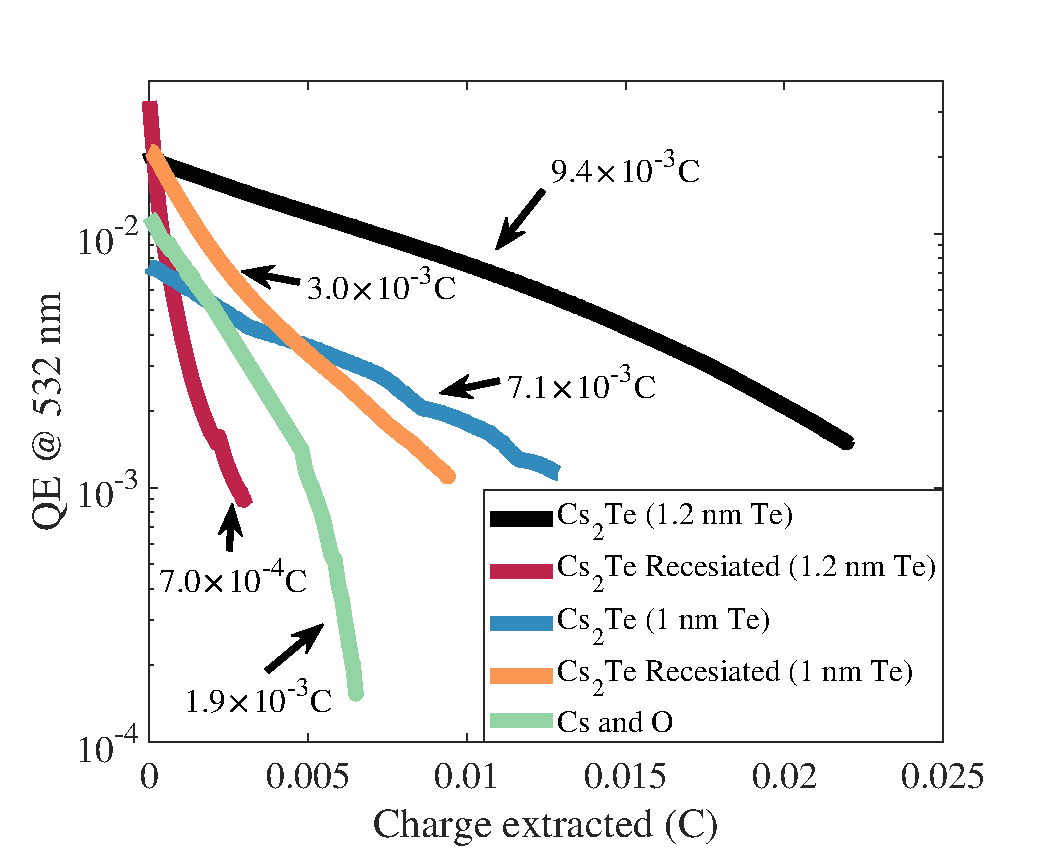
\includegraphics[scale=0.53]{figs/CsTe/lifetime.eps}
    \caption{Quantum Efficiency of GaAs with various surface conditions at 532 nm wavelength as a function of extracted charges. The number next to each curve is the charge lifetime obtained from an exponential fit.
    %An exponential fit to each curve is used to retrieve charge lifetimes for each sample.
    }
    \label{lifetime}
\end{figure}
% mott

The photocathode laboratory UHV installation has been upgraded with a low energy reflection mode Mott polarimeter that was originally part of SLAC photocathode test-stand.\cite{alley1995_StanfordLinearAccelerator} This Mott analyzer's Sherman function was characterized to be $S_\mathrm{eff}=0.15$ at 20 kV operating voltage with a 5\% accuracy when electrons within a 1 keV energy loss window are allowed to be detected.\cite{Mulhollan_SLAC}
Monochromatic light was circularly polarized using a linear polarizer (Thorlabs LPVIS050) and a liquid crystal variable wave plate (Thorlabs LC1113B), and it was directed unto the sample surface at normal incidence. The helicity of circular polarization was switched by alternating retardance of the liquid crystal wave plate between $\frac{1}{4}\lambda$ and $\frac{3}{4}\lambda$. %Generated optical circular polarization was measured to be higher than 99\% for both helicity states over the spectral range between 600 and 900 nm.

One of GaAs samples was first activated to NEA using Cs and O$_2$, and then moved into the UHV chamber equipped with the Mott polarimeter. Photoelectrons were transported to the Mott detector, and from the measured asymmetries in the scattering process and the known value of the $S_\mathrm{eff}$, the electron beam polarization was obtained for different wavelengths. See Figure \ref{pol}. The measured values agree quite well with those recently reported for similar bulk GaAs by another group.\cite{liu2017_ComprehensiveEvaluationFactors} The same sample was then moved back to the Cs$_2$Te growth chamber. There it was first heated for 12 hours at 400~$^\circ$C to remove the Cs and O$_2$ from its surface, and then Cs$_2$Te thin film was deposited on it. Once the GaAs sample was activated with Cs$_2$Te, it was moved back to the Mott chamber to measure the spin polarization of photoelectrons. Results are reported in Figure \ref{pol} as well. We found that the Cs$_2$Te thin film did not affect the polarization of the photoelectrons from GaAs.


% Depolarization mechanism + polarization result
Although the maximum theoretical electron spin polarization achievable for bulk GaAs is 50\%, due to spin relaxation mechanisms happening before the emission into vacuum, 30-40\% degree of polarization is usually attained from NEA GaAs. For GaAs, electron spin relaxation mechanisms have been extensively studied and are dominated by the lack of inversion symmetry and the exchange interaction between electrons and holes, leading to a characteristic relaxation time $\tau_s$ of $\sim$100 ps at room temperature.\cite{fishman1977_SpinRelaxationPhotoelectrons,zutic2004_SpintronicsFundamentalsApplications,song2002_SpinRelaxationConduction}
Additional depolarization mechanisms at activation layers are relatively unknown and have been considered negligible because the Cs and O$_2$ activation is on the order of less than a monolayer. In case of Cs$_2$Te activation layer, the thickness might be no longer negligible and the activation layer can become an additional source of spin depolarization.
%According to the predicted Cs$_2$Te electronic structure,\cite{DFT} the effective mass in the conduction band is 1.1$m_e$.
Based on Refs.~\cite{zutic2004_SpintronicsFundamentalsApplications,song2002_SpinRelaxationConduction}, we estimate $\tau_s$ to be similar to that of GaAs but dominated by the lack of inversion symmetry and the spin-orbit coupling, due to a heavier electron effective mass. The conduction band electron effective mass of 1.1$m_e$ at $\Gamma$ point was used based on calculations.\cite{terdik2012_AnomalousWorkFunction} From this estimate, we expect that electrons can travel several tens of nm in Cs$_2$Te without experiencing significant depolarization. Our results reported in Figure~\ref{pol} support this conclusion.

An electron mean free path of 3\,nm and mean energy losses of 5\,meV have been used to accurately reproduce the spectral response of Cs$_2$Te using Monte Carlo techniques.\cite{ferrini_MONTECARLOSIMULATION} Assuming 0.15\,eV as the maximum energy of electrons excited in GaAs with 780\,nm light and injected into the Cs$_2$Te layer (see Figure \ref{levels}): electrons should still be able to escape even after having experienced on the order of 30 ($=0.15\,\mathrm{eV}/5\,\mathrm{meV}$) scattering events. Making the assumption of small scattering angles,\cite{jacoboni1989_MonteCarloMethod} a few tens of nm of Cs$_2$Te should also not drastically affect the efficiency of electron emission. 

\begin{figure}
    \centering
    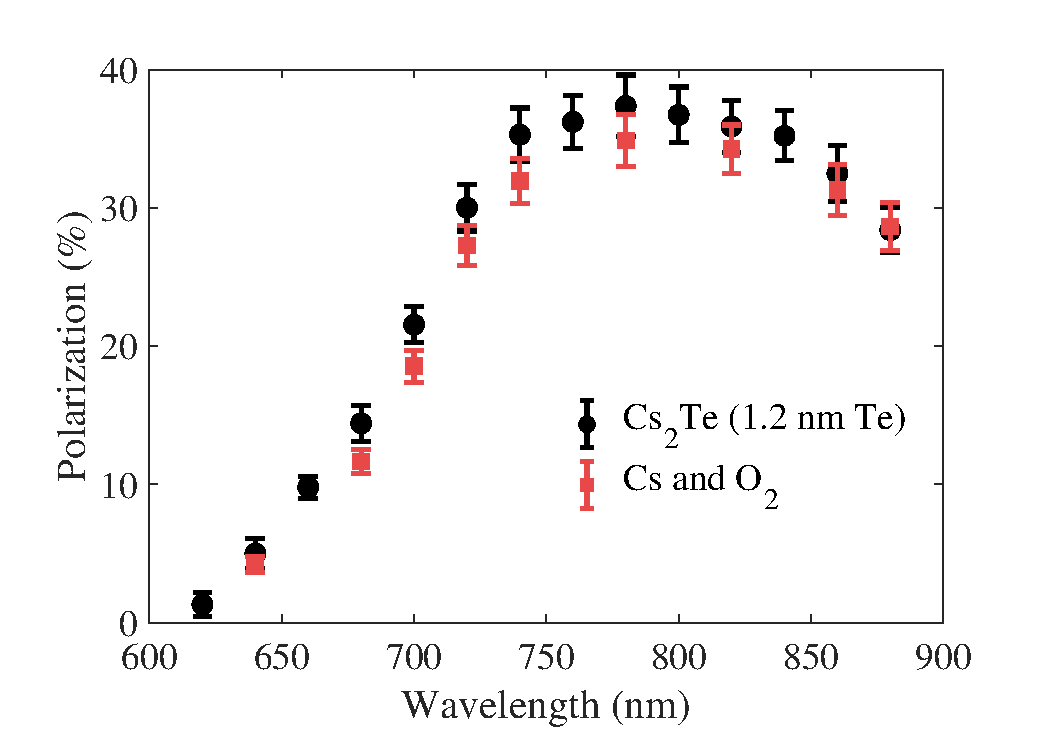
\includegraphics[scale=0.53]{figs/CsTe/pol.eps}
    \caption{Spin polarization measured from GaAs samples activated by Cs$_2$Te and Cs and O$_2$ as a function of the laser wavelength. %Uncertainty of the measure is dominated by statistical errors.
    }
    \label{pol}
\end{figure}

In conclusion, we activated GaAs with Cs$_2$Te for studying its effect on NEA formation, lifetime, and spin-polarization of the photocathode. NEA condition was confirmed by the spectral response. The lifetime showed a factor of 5 improvement while the spin polarization remained the same as the one obtained with the Cs and O$_2$ standard activation.
Based on our presented results and simplified estimates predicting negligible losses of quantum efficiency and spin polarization, we plan to experiment with a thicker Cs$_2$Te to further improve the photocathode lifetime.
We believe that our work triggers a paradigm shift on activating GaAs photocathodes with other materials that can both form more robust NEA activation layers and enable applications requiring high spin-polarized photoelectrons.

This work is supported by DOE Grant No. DE-SC0016203 and NSF PHY-1461111. The authors wish to acknowledge T. Maruyama, M. Stuzman, and M. Poelker for fruitful discussions and help in recommissioning the Mott polarimeter.
